\section{Introduction}

Current Supercomputing Centers (SCs) for High-Performance Computing (HPC) with peta-scale capabilities have high power demands, with peak requirements of over 30 MW and fluctuations of a few megawatts. This trend is expected to continue in the future as we push the limits of supercomputing further. As a result, Electricity Service Providers (ESPs) for such SCs need to support efficient electricity generation, transmission and distribution along with reliable grid operation. ESPs today already face reliability concerns for accommodating megawatt-level fluctuations from SCs and often require HPC client sites to forecast their electricity use. The acceptance and proliferation of renewable sources of energy further adds to the variability at the electricity generation end, making grid reliability even more challenging. A tighter integration and open communication between ESPs and their client SCs is thus critical as we proceed toward the next generation of supercomputing. \\

At present, most ESP-SC relationships are linear and unidirectional. Power is typically generated, distributed and delivered to customer sites without direct active involvement, and most electricity pricing contracts are negotiated without tight integration requirements. Going forward, however, it is expected that a multi-directional relationship will evolve between the ESPs and SCs.  Communication and control will flow from end-customers to one or more of the electricity generation and distribution entities, and contract terms will enforce stringent usage requirements. The cloud and data center providers, such as Google, have already started to anticipate this multi-directional relationship and are taking advantage of this changing landscape.  For example, Google's response suggests vertical integration, especially with Google's Energy Subsidiary which gives Google the right to sell energy within the United States. (need citation). Another example is the SmartGrid initiative \cite{SmartGrid} by the U.S. Department of Energy, which is making electricity delivery faster and more efficient by involving customers, adjusting to dynamic demands, and by providing automated solutions and quick responses to remote locations. Techniques involved in establishing such multi-directional relationships are referred to as \emph{demand management} (DM) techniques. The Energy-Efficient High-Performance Computing Working Group (EE HPC WG) seeks to analyze the impact of similar DM techniques for SCs with HPC workloads and their ESPs. \\

In our previous work, we focused on understanding how ESPs and SCs can work together to improve energy efficiency by surveying large-scale SCs in the United States \cite{BatesESP}. We developed a questionnaire and noted that none of the SCs are working directly with their ESPs. Our main conclusion from this work was that SCs in the United States were interested in a tighter integration with their ESPs, but a business case for the same had not been demonstrated. In this work, we expand our analysis to include European SCs, where electricity is more expensive and is subject to more variability because of the use of renewable sources of energy. We expected that the European SCs would be more tightly integrated with their ESPs because of the higher prices and more extensive use of renewables in Europe.  Contrary to our expectations, however, we found that the United States shows more interest in responding to requests from their ESPs than Europe.  There are four 10+MW SCs in the United States, whereas all of the remaining SCs in both the United States and Europe are 5MW or less.  These four 10+MW SCs have all had communication with their ESPs about responding to grid requests.  Perhaps they are harbingers for the lower power demand SCs.  Another factor explaining the difference may be greater availability of electricity demand response incentive programs in the United States than in Europe. In future studies, we hope to better understand the European ESPs and their environment to see if this hypothesis has merit. 

An example of this can be seen in Figure \ref{fig:seq}, which depicts the fluctuations in megawatts on the world's third fastest supercomputer, Sequoia, which delivers 16.3 petaflops and is hosted at Lawrence Livermore National Laboratory.

%There is a movement away from a linear, uni-directional system where power is generated, distributed and delivered to customers without their involvement.  The evolving system is multi-directional (or at least bi-directional) with communication and control going from end-customers to one or more of the electricity generation and distribution entities.  The cloud providers, like Google, have already started to anticipate and take advantage of this changing landscape.  Google's response suggests vertical integration, especially with Google's Energy Subsidiary which gives Google the right to sell energy within the United States.  It is thus critical to understand the relationship between SCs and their associated Electricity Service Providers (ESPs) and to encourage the development of a more symbiotic association between the two. More specifically, it is important to analyze the expectations of SCs and ESPs from each other, and to study the willingness and feasibility of grid integration techniques. For example, the SmartGrid initiative \cite{SmartGrid} by the U.S. Department of Energy is making electricity delivery more fast and efficient by involving customers, adjusting to dynamic demands, and providing automated solutions and quick responses to remote locations. T
\begin{figure}
\begin{center}
\frame{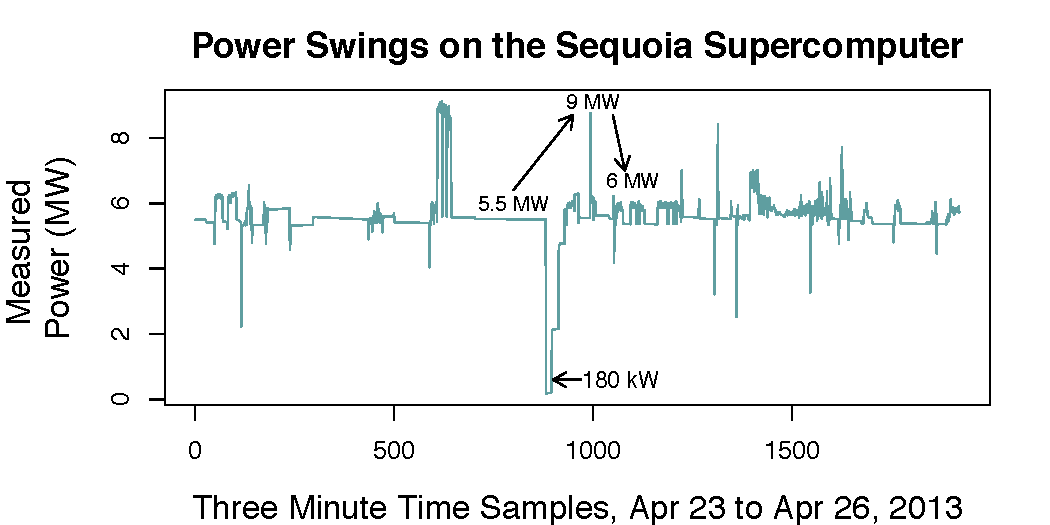
\includegraphics[scale=0.6]{figs/seq.pdf}}
\caption{Sequoia Supercomputer Power Swings}
\label{fig:seq}
\end{center}
\end{figure}



We accomplished expanding our analysis to Europe by extending the aforementioned questionnaire to European SCs. Nine out of the sixteen SCs that we contacted responded to the questionnaire. All except one of these sites were in Top 50 supercomputers in the world \cite{Top500}. Section \ref{res} presents an overview of our results from the questionnaire. Section \ref{spm} discusses the strategies, programs and methods that were used in the questionnaire and the willingness of respondents to consider these options. Section \ref{comm} highlights some of the comments we received from our respondents, and Section \ref{summary} concludes this article.
